\section*{Потоки и разрезы}
\begin{enumerate}
	\item Дан граф и выделенные вершины $s, t$. Нужно проверить, правда ли существует единственный минимальный s-t разрез.
	\begin{enumerate}
		\item $O(poly(V, E))$
		
		\textbf{Решение.} Заметим, что минимальный $s-t$ разрез мы можем найти при помощи алгоритма 
		Форда-Фалкерсона, указав пропускную способность каждого ребра равной единице (Обозначим размер 
		минимального разреза $F$). Если таких минимальных разрезов несколько, то увеличив до 2 пропускную 
		способность какого-то из рёбер мин. разреза, мы получим другой разрез с потоком $F$. Осталось понять, 
		какому ребру нужно уменьшать пропускную способность (нужно выбрать то, которое входит в один мин. разрез, 
		и не входит в другой). Раз уж мы не очень ограничены в сложности, то переберём все ребра исходного мин. 
		разреза(их не более $E$), уменьшим пропускную способность каждого из рёбер, заново найдём поток, если он 
		равен $F$, то разрез не единственный, если после уменьшения пропускной способности всех рёбер поток 
		уменьшался, то 
		минимальный $s-t$ разрез в исходном графе единственен. Сложность описанного подхода, очевидно, $O(poly(V, E))$
		\item $O(E)$ при условии, что нам уже известен максимальный поток (с доказательством).
		
		\textbf{Решение.} Рассмотрим остаточную сеть, для известного нам максимального потока. Найдём множество 
		вершин $S$ - все вершины, достижимые по ребрам остаточной сети из вершины $s$, $T$ - все вершины 
		остаточной сети, которые достижимы из $t$ по обратным ребрам. Заметим, что разрезы $[S, V/S]$ и $[V/T, 
		T]$ - минимальные. Если они различны, то минимальный разрез не единственный. 
		
		Покажем, что если они совпадают, то минимальный разрез $C$ будет единственным. Предположим противное, и 
		существует другой разрез $\hat{C}$. Но тогда существует путь из $s$ в $t$ содержащий ребро $e = (v, u) 
		\in \hat{C}$. Рассмотрим вершину $v$ - ближайшую к $s$. Заметим, что пути в остаточной сети из $s$ в $v$ 
		нет, т.к. они отделены разрезом $C$, с другой стороны, нет пути и из $v$ в $t$ по остаточным ребрам. 
		Поэтому $v\notin S \land v \notin T \Rightarrow V /T \neq S$ - противоречие. Значит, если разрезы 
		совпали, то других разрезов быть не может.
		
		Таким образом, мы научились за сложность $O(DFS)$ проверять единственность мин. разреза. Это и есть 
		$O(E)$.
	\end{enumerate}
	
	\item В неориентированном графе без кратных рёбер необходимо удалить минимальное число рёбер так, чтобы 
	увеличилось количество компонент связности. $O(V \cdot Flow)$. Оцените время работы	того же алгоритма более 
	точно как $O(E^2)$.
	
	% TODO: описать способ ориентации ребер графа.
	
	\textbf{Решение.} Сразу скажем, что для решения задачи достаточно научиться искать мин. количество рёбер, 
	которое нужно удалить чтобы развалить граф для связных графов, т.к. для несвязных достаточно предпосчитать 
	компоненты связности за $O(DFS) = O(V + E)$, а потом искать минимальные разрезы для каждой компоненты. 
	Сложность при этом не изменится.
	
	Будем искать минимальные разрез следующим образом. Рассмотрим некоторый минимальный разрез для исходного 
	графа. Он разобьёт множество вершин графа на две непустые части: $S, V / S$. Теперь заметим, 
	что для того, чтобы найти этот разрез достаточно выбрать в качестве вершины истока некоторую вершину $s \in 
	S$, а в качестве вершины - стока $t \in V / S$, после чего лишь останется всем рёбрам дать пропускную 
	способность, равную единице, и найти максимальный поток. Осталось понять, как выбрать вершины $s, t$. 
	Это можно сделать так: $s$ выберем произвольно, $t$ переберём все остальные. Хотя бы одно значения 
	$t$ окажется в другой части разбиения множества вершин графа, и именно в этом случае мы и получим минимальный 
	разрез. То есть нужно запустить $V - 1$ алгоритм поиска максимального потока. А заметив, что ребра графа 
	имеют пропускные способности равные единице, можем получаем возможность искать максимальный поток за $O(VE)$. 
	Т.к. кратных рёбер нет, то $V^2 = O(E)$, значит итоговую сложность можно оценить как $O(V^2E) = O(E^2)$. 
	
	\item Есть ориентированный граф с начальной и конечной вершинами. В начальной вершине есть $K$ грузовиков. 
	Грузовикам нужно попасть в конечную вершину. Время дискретно. За единицу времени каждый грузовик или стоит на 
	месте, или перемещается в одну из соседних вершин. В любой вершине могут одновременно стоять несколько 
	грузовиков. По любому из рёбер в каждый момент времени должен ехать не более чем один грузовик. Минимизируйте 
	время, когда все грузовики окажутся в конечной вершине.
	\begin{enumerate}
		\item $O(poly(V, E, K))$
		Для начала заметим, что время, которого будет достаточно, чтобы все грузовики переехали из начальной 
		точки в конечную не превосходит $V + K$ - т.к. макс. длина кратчайшего пути $V$, и нужно переправить $K$ 
		грузовиков. Тогда можно простроить орграф из $V + K$ слоёв и искать в нем макс. поток. 
		
		Слой графа представляет собой вершины исходного графа. Рёбер внутри слоя между ними нет. А дискретный 
		переход на следующий момент времени соответствует переходу на следующий слой. То есть каждая вершина $v$ 
		заменится на $V + K$ вершин $v_1, v_2, ..., v_{V + K}$. 
		
		Добавим ребра-переходы между слоями. Если в графе между вершинами $u, v$ было ребро, то нужно добавить 
		ребра между всем соседними слоями $u_{i} \to v_{i + 1}$, причём пропускную способность этого ребра 
		сделаем равной единице - что соответствует, что в $i$-ый момент времени только один грузовик может 
		переехать из вершины $u$ в вершину $v$. Заметим, что грузовикам разрешает оставаться в той же вершине. 
		Это значит, что нужно добавить ребра $(v_i, v_{i + 1})$ с пропускной способностью $K$ - сколько угодно 
		грузовиком могут остаться в той же вершине.
		
		Обозначим $s$ - начальная вершина, $t$ - конечная. Заметим, что теперь величина максимального потока из 
		$s_1$ в $t_n$ соответствует сколько максимум грузовичков могут добраться из начальной вершины в конечную 
		за время $n$. Значит нам осталось просто найти такое минимальное $n$, при котором величина максимального 
		потока из $s_1$ в $t_n$ будет равна хотя бы $K$. 
		
		Сложность при таком подходе, $O(poly(V, E, K))$, т.к. мы ищем не более чем $V + K$ раз максимальный поток 
		в графе, в котором $V(V + K)$ вершин, и $O((E + V)(V + K))$ ребер.
		\item $O(K(V + K)E)$
		
		\textbf{Решение.} Заметим что в пункте $(a)$ поток был не ограничен. Можем его ограничить добавив новую 
		вершину - исток, и соединив её ребром с вершиной $s_1$ с пропускной способностью $K$. Теперь величина 
		потока не может превосходить $K$. Можем среди вершин $t_1, t_2, ... , t_{V+K}$ бинарным поиском минимальное 
		$n$, такое, что поток $s\to t_n$ равен $K$. Сложность при этом подходе составит $O((V+K)E K \log(V + K))$.  
		Избавимся от логарифма тем же приемом как и в задаче 3 в классе, пересчитав поток от $t_i$ к $t_{i + 1}$.
		
		Получим требуемую сложность $O(K(V + K)E)$.
	\end{enumerate}
	
	\item Есть $n$ рабочих и $m$ работ. И есть матрица умения: <<какой рабочий какие работы умеет делать>>. Нужно 
	максимально равномерно распределить работы между рабочими. То есть, каждой работе сопоставить рабочего, который 
	умеет делать эту работу, а кроме того минимизировать $\max\limits_{i=1\dots n} k_i$ где $k_i$ – количество 
	работ, выданных $i$-му рабочему.
	
	\textbf{Решение.} Построим следующую сеть $N(k)$. Выпишем в столбец $n$ рабочих, справа от них выпишем в 
	столбец $m$ работ. Соединим рабочего со всеми работами, которые он умеет делать, пропускную способность 
	этого ребра установим равной единице. Добавим слева от рабочих исток, справа от работ сток. Соединим каждую 
	работу со стоком ребром пропускной способности $1$. А исток с каждым из рабочих ребром пропускной 
	способностью $k$, где $k$ - параметр сети. Очевидно, что максимальная величина потока в сети равна $m$, это 
	соответствует случаю, когда каждую из работ выполняет какой-то рабочий.
	
	Теперь осталось найти такое значения $k$, что величина максимального потока для сети $N(k)$ равна $m$, но 
	величина максимального потока для сети $N(k - 1) < m$. То есть мы находим такое значения $k$, которое 
	позволяет выдать каждому рабочему не более $k$, работ, но при котором все работы могут быть выполнены. Это и 
	есть ответ на исходную задачу.
	
	Про сложность тут ничего не сказано, поэтому можно просто перебирать значения $k$ от $1..m$, до тех пор, 
	пока величина потока не станет равна $m$. При желании можно ускорить, используя бинарный поиск.
\end{enumerate}

\subsection*{Дополнительные задачи}
\begin{enumerate}
	\item[2.] Найдите ориентированный граф с целочисленными пропускными способностями, на которых детерменированный 
	алгоритм Форда-Фалкерсона на основе $DFS$ с фиксированным порядком просмотра рёбер в каждой вершине, 
	пропускающий максимум по дополняющему пути, работает за экспоненту от $V$.
	
	\textbf{Решение.} На лекции был пример со стучаем, когда алгоритм Форда-Фалкерсона работает долго, его можно 
	индуктивно расширить, экспоненциально увеличивая время работы, но добавляя от шага к шаге лишь 2 вершины.
	\begin{center}
		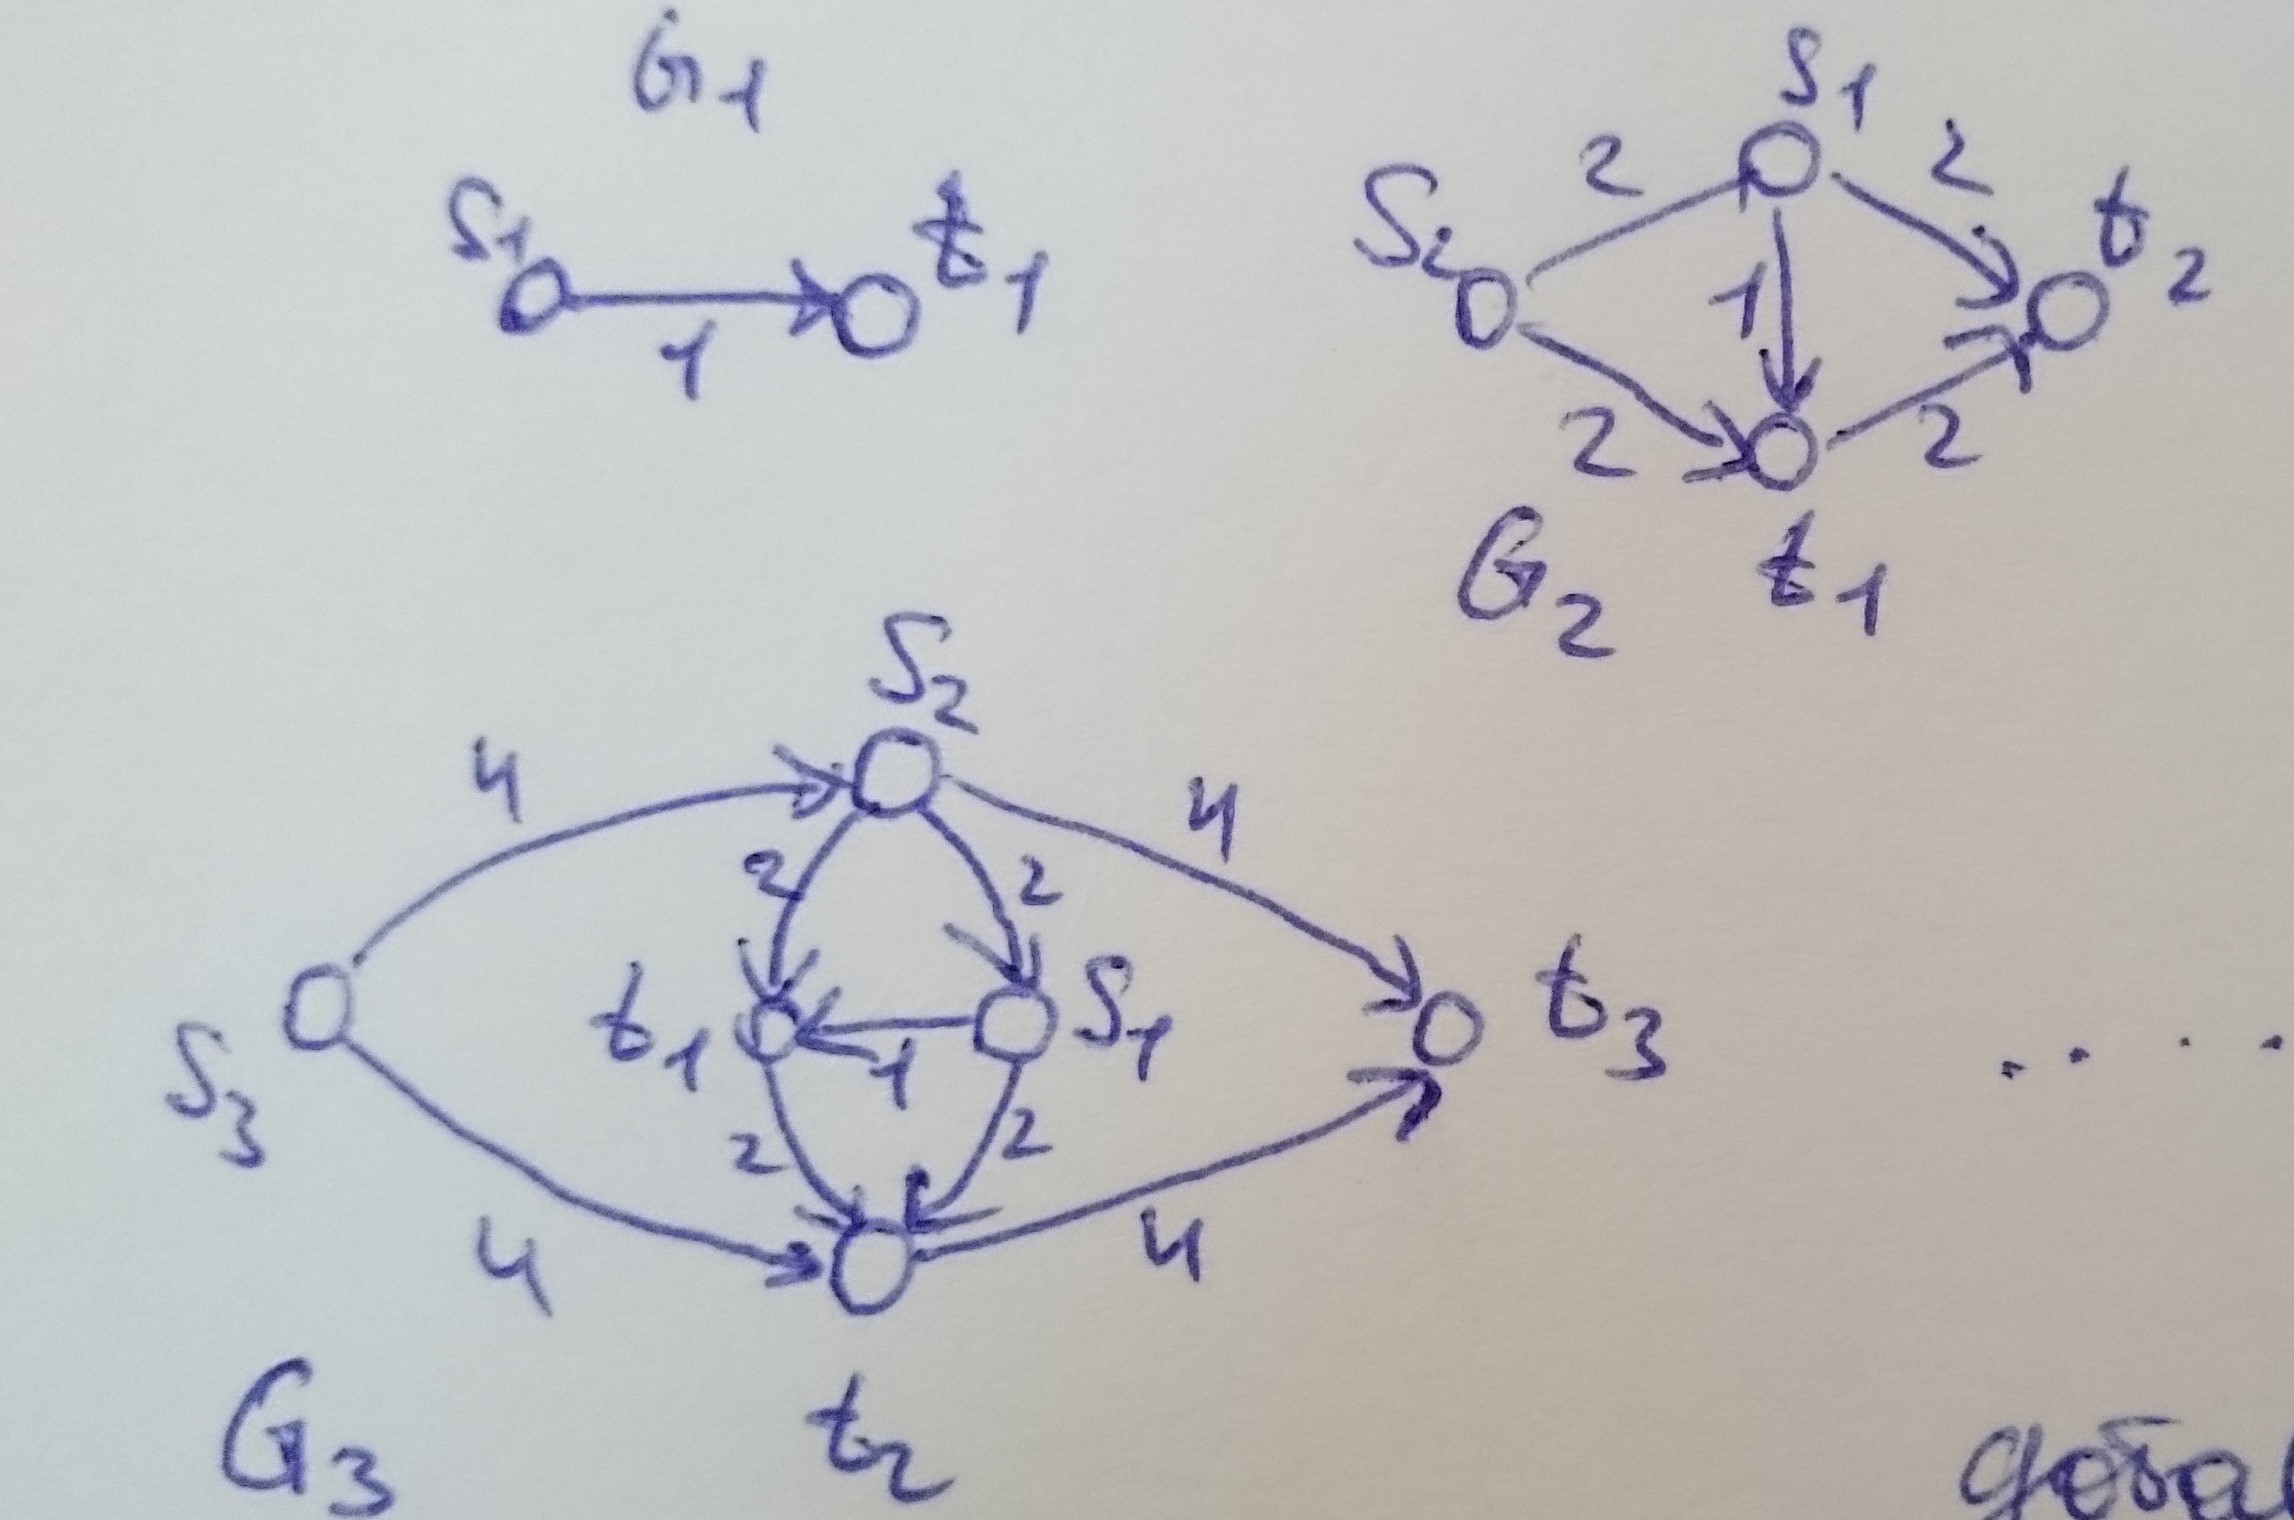
\includegraphics[scale=0.1]{ha/img/1.JPG}
	\end{center}
	То есть если $dfs$ после прохода по ребру будет заходить каждый раз в подграф меньшего размера, то за $1$ 
	итерацию поток будет увеличиваться только на единицу. И установив, вес новых рёбер как степени двойки мы 
	добьёмся экспоненциальной сложности работы алгоритма.
\end{enumerate}